% Created 2016-08-17 Wed 14:38
\documentclass[tikz]{standalone}

\usepackage[utf8]{inputenc}
\usepackage[T1]{fontenc}

\usepackage{circledsteps}

\RequirePackage{xcolor}

%% HPI color definitions according to the design manual
% These do not exactly match the RGB values used in the Powerpoint slide master due to unknown reasons
\definecolor{hpiyellow}{RGB}{246,168,0}
\definecolor{hpiorange}{RGB}{221,97,8}
\definecolor{hpired}{RGB}{177,6,58}
\definecolor{hpigray}{RGB}{90,96,101}
\definecolor{hpiblue}{RGB}{0,122,158}


\renewcommand{\sfdefault}{neosans}
% Different font weights for neosans
\newcommand{\textl}[1]{{\fontseries{l}\selectfont #1}} % light
\newcommand{\textm}[1]{{\fontseries{m}\selectfont #1}} % medium, same as default weight
\newcommand{\textsb}[1]{{\fontseries{sb}\selectfont #1}} % semibold
\newcommand{\textmb}[1]{{\fontseries{mb}\selectfont #1}} % bold, same as \textbf
\newcommand{\texteb}[1]{{\fontseries{eb}\selectfont #1}} % extra bold
\newcommand{\textub}[1]{{\fontseries{ub}\selectfont #1}} % ultra bold

\tikzset{every picture/.style={/utils/exec={\sffamily}}}
\tikzset{flipflop RSflanke/.style={
  flipflop,
  flipflop def={t1=S, t2=C, c2=1, t3=R, t6=Q, t4={\ctikztextnot{Q}}}
}}


\tikzset{
  mechanicalSwitch/.pic={
    \coordinate (-inUp) at (135:2); 
    \coordinate (-inDown) at (235:2);
    \coordinate (-out) at (2,0);
    \coordinate (-center) at (0,0);
    
    \draw (0,0) circle [radius = 2cm];
    \draw [fill=gray!20] (0,0) circle [radius = 0.2cm];

    \draw (0, 0) -- (2, 0);
    \draw (135:.8) -- (135:2); 
    \draw (225:.8) -- (225:2); 

    \draw [fill=gray!20] (2, 0) circle [radius=0.05cm]; 
    \draw [fill=gray!20] (135:2) circle [radius=0.05cm]; 
    \draw [fill=gray!20] (225:2) circle [radius=0.05cm]; 

    
    \draw [thick] (0,0) -- (175:1.5); 

    \draw [dashed, <->, domain=135:225] plot ({cos(\x)}, {sin(\x)}); 
  },
  mechanicalSwitchClosed/.pic={
    \coordinate (-inUp) at (135:2); 
    \coordinate (-inDown) at (255:2);
    \coordinate (-out) at (2,0);
    \coordinate (-center) at (0,0);
    \draw (0,0) circle [radius = 2cm];
    \draw [fill=gray!20] (0,0) circle [radius = 0.2cm];

    \draw (0, 0) -- (2, 0);
    \draw (135:.8) -- (135:2); 
    \draw (225:.8) -- (225:2); 

    \draw [fill=gray!20] (2, 0) circle [radius=0.05cm]; 
    \draw [fill=gray!20] (135:2) circle [radius=0.05cm]; 
    \draw [fill=gray!20] (225:2) circle [radius=0.05cm]; 

    
    \draw [thick] (0,0) -- (135:2); 

    \draw [dashed, <->, domain=135:225] plot ({cos(\x)}, {sin(\x)}); 
  }
}


\usetikzlibrary{calc}
\usetikzlibrary{positioning}


\usepackage{pgfplots}

\begin{document}

\begin{tikzpicture}
  \label{page:phy:ascii_b}
  \begin{axis}[no markers,
    xlabel={Time/s},
    ylabel=Voltage,
    ]
    \addplot coordinates { (0,0) (1,0) (1,1) (3,1) (3,0) (6,0) (6,1) (7,1) (7,0) (8,0)};
  \end{axis}
\end{tikzpicture}


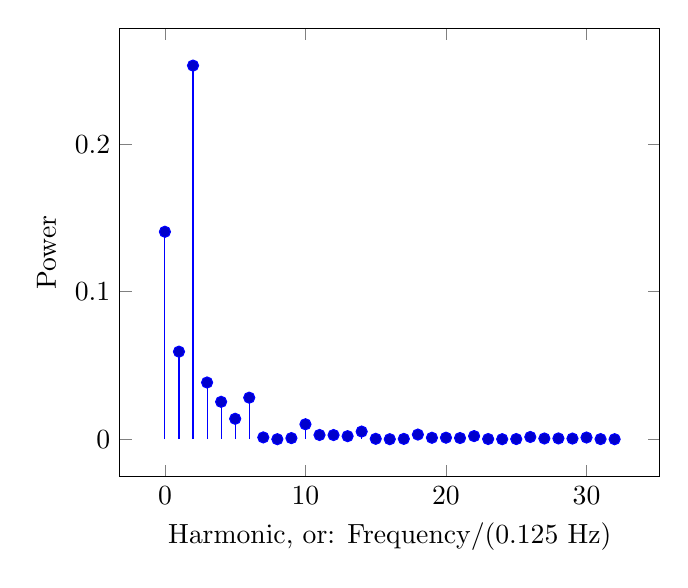
\begin{tikzpicture}
  \label{page:phy:spectrum:ascii_b}
  % compare fourier2.py 
  \begin{axis}[xlabel={Harmonic, or: Frequency/(0.125 Hz)}, ylabel=Power, ycomb]
    \addplot table {
0	0.140625
1	0.05935257522198646
2	0.2533029591058445
3	0.03843690659415164
4	0.025330295910584447
5	0.013837286373894609
6	0.028144773233982703
7	0.0012112770453466552
8	8.547605795164205e-34
9	0.0007327478422467396
10	0.010132118364233795
11	0.002858943465680698
12	0.002814477323398272
13	0.0020469358541264247
14	0.005169448145017245
15	0.0002637892232088291
16	8.547605795164205e-34
17	0.00020537223260202791
18	0.003127197025998091
19	0.0009582608292170749
20	0.0010132118364233778
21	0.0007844266651867665
22	0.0020934128851722708
23	0.00011219768472965265
24	4.225307908614651e-33
25	9.496412035517814e-05
26	0.0014988340775493796
27	0.00047452971103891103
28	0.0005169448145017233
29	0.0004113343155141102
30	0.001125790929359308
31	6.17612645390098e-05
32	8.547605795164205e-34
% 33	5.450190562165972e-05
% 34	0.0008764808273558644
% 35	0.0002823935994672348
% 36	0.000312719702599808
% 37	0.0002526896708161943
% 38	0.0007016702468305893
% 39	3.9022074439176394e-05
% 40	8.547605795164205e-34
% 41	3.5307897217124204e-05
% 42	0.0005743831272241365
% 43	0.00018709148693745814
% 44	0.0002093412885172269
% 45	0.0001708306959740063
% 46	0.0004788335710885535
% 47	2.6868526583064717e-05
% 48	4.225307908614651e-33
% 49	2.4719939700952473e-05
% 50	0.000405284734569351
% 51	0.00013299967679636935
% 52	0.0001498834077549375
% 53	0.00012315135612223785
% 54	0.00034746633622200526
% 55	1.962068602379961e-05
% 56	3.640016494805606e-32
% 57	1.8267951745763766e-05
% 58	0.0003011925791983916
% 59	9.937723623882883e-05
% 60	0.00011257909293593089
% 61	9.29675246835149e-05
% 62	0.00026358268377298826
% 63	1.4954037596871867e-05
% 64	8.547605795164205e-34
};
  \end{axis}
\end{tikzpicture}

\begin{tikzpicture}
  \begin{axis}[no markers,
    xlabel={Time/s},
    ylabel=Voltage,
    domain=0:8,
    ]
    \addplot coordinates { (0,0) (1,0) (1,1) (3,1) (3,0) (6,0) (6,1) (7,1) (7,0) (8,0)};
    \addplot expression {3/4}; 
  \end{axis}
\end{tikzpicture}


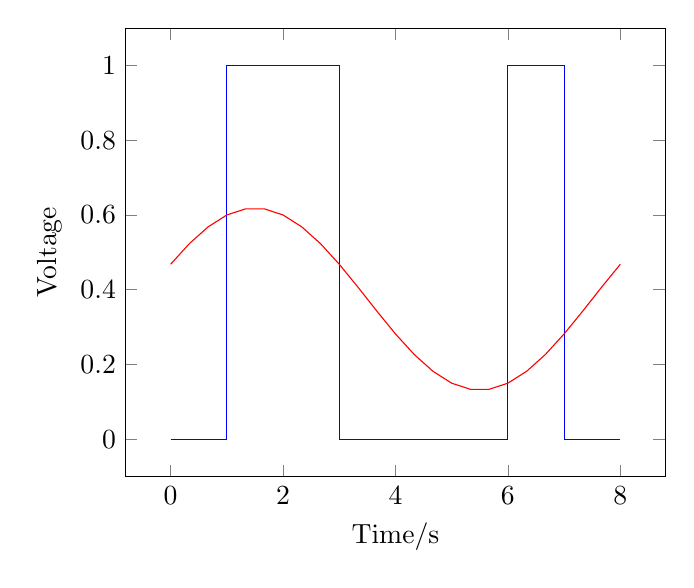
\begin{tikzpicture}
  \begin{axis}[no markers,
    xlabel={Time/s},
    ylabel=Voltage,
    domain=0:8,
    trig format plots=rad,
    ]
    \addplot coordinates { (0,0) (1,0) (1,1) (3,1) (3,0) (6,0) (6,1) (7,1) (7,0) (8,0)};
    \addplot expression {1/2*3/4 + % 
      % a1:
      1/(pi*1) * ( cos (pi * 1/4) - cos (3*pi *1 /4) + cos (6*pi* 1/4) - cos(7*pi*1/4)) * sin(2*pi* 1* 1/8 * x)  + % 
      % b1:
      1/(pi * 1) * (sin (3*pi * 1/4) - sin(pi *1/4) + sin (7*pi * 1/4) - sin (6*pi*1/4) ) * cos(2*pi* 1 * 1/8*x)
     }; 
  \end{axis}
\end{tikzpicture}


% \begin{tikzpicture}
%   \begin{axis}[no markers,
%     xlabel={Time/s},
%     ylabel=Voltage,
%     domain=0:8,
%     trig format plots=rad,
%     samples=100,
%     ]
%     \addplot coordinates { (0,0) (1,0) (1,1) (3,1) (3,0) (6,0) (6,1) (7,1) (7,0) (8,0)};
%     \addplot expression {1/2*3/4 + % 
%       % a1:
%       1/(pi*1) * ( cos (pi * 1/4) - cos (3*pi *1 /4) + cos (6*pi* 1/4) - cos(7*pi*1/4)) * sin(2*pi* 1* 1/8 * x)  + %
%       % a2: 
%       1/(pi*2) * ( cos (pi * 2/4) - cos (3*pi * 2 /4) + cos (6*pi* 2/4) - cos(7*pi*2/4)) * sin(2*pi* 2 * 1/8 * x)  + %
%       % b1:
%       1/(pi * 1) * (sin (3*pi * 1/4) - sin(pi *1/4) + sin (7*pi * 1/4) - sin (6*pi*1/4) ) * cos(2*pi* 1 * 1/8*x) + %
%       % b2:
%       1/(pi * 2) * (sin (3*pi * 2/4) - sin(pi *2/4) + sin (7*pi * 2/4) - sin (6*pi*2/4) ) * cos(2*pi* 2 * 1/8*x)  %
%      }; 
%   \end{axis}
% \end{tikzpicture}


% \begin{tikzpicture}
%   \begin{axis}[no markers,
%     xlabel={Time/s},
%     ylabel=Voltage,
%     domain=0:8,
%     trig format plots=rad,
%     samples=100,
%     ]
%     \addplot coordinates { (0,0) (1,0) (1,1) (3,1) (3,0) (6,0) (6,1) (7,1) (7,0) (8,0)};
%     \addplot expression {1/2*3/4 + % 
%       % a1:
%       1/(pi*1) * ( cos (pi * 1/4) - cos (3*pi *1 /4) + cos (6*pi* 1/4) - cos(7*pi*1/4)) * sin(2*pi* 1* 1/8 * x)  + %
%       % a2: 
%       1/(pi*2) * ( cos (pi * 2/4) - cos (3*pi * 2 /4) + cos (6*pi* 2/4) - cos(7*pi*2/4)) * sin(2*pi* 2 * 1/8 * x)  + %
%       % a3: 
%       1/(pi*3) * ( cos (pi * 3/4) - cos (3*pi * 3 /4) + cos (6*pi* 3/4) - cos(7*pi*3/4)) * sin(2*pi* 3 * 1/8 * x)  + %
%       % b1:
%       1/(pi * 1) * (sin (3*pi * 1/4) - sin(pi *1/4) + sin (7*pi * 1/4) - sin (6*pi*1/4) ) * cos(2*pi* 1 * 1/8*x) + %
%       % b2:
%       1/(pi * 2) * (sin (3*pi * 2/4) - sin(pi *2/4) + sin (7*pi * 2/4) - sin (6*pi*2/4) ) * cos(2*pi* 2 * 1/8*x) +  %
%       % b3:
%       1/(pi * 3) * (sin (3*pi * 3/4) - sin(pi *3/4) + sin (7*pi * 3/4) - sin (6*pi*3/4) ) * cos(2*pi* 3 * 1/8*x) %
%      }; 
%   \end{axis}
% \end{tikzpicture}


% \begin{tikzpicture}
%   \begin{axis}[no markers,
%     xlabel={Time/s},
%     ylabel=Voltage,
%     domain=0:8,
%     trig format plots=rad,
%     samples=100,
%     ]
%     \addplot coordinates { (0,0) (1,0) (1,1) (3,1) (3,0) (6,0) (6,1) (7,1) (7,0) (8,0)};
%     \addplot expression {1/2*3/4 + % 
%       % a1:
%       1/(pi*1) * ( cos (pi * 1/4) - cos (3*pi *1 /4) + cos (6*pi* 1/4) - cos(7*pi*1/4)) * sin(2*pi* 1* 1/8 * x)  + %
%       % a2: 
%       1/(pi*2) * ( cos (pi * 2/4) - cos (3*pi * 2 /4) + cos (6*pi* 2/4) - cos(7*pi*2/4)) * sin(2*pi* 2 * 1/8 * x)  + %
%       % a3: 
%       1/(pi*3) * ( cos (pi * 3/4) - cos (3*pi * 3 /4) + cos (6*pi* 3/4) - cos(7*pi*3/4)) * sin(2*pi* 3 * 1/8 * x)  + %
%       % a3: 
%       1/(pi*4) * ( cos (pi * 4/4) - cos (3*pi * 4/4) + cos (6*pi* 4/4) - cos(7*pi*4/4)) * sin(2*pi* 4 * 1/8 * x)  + %
%       % b1:
%       1/(pi * 1) * (sin (3*pi * 1/4) - sin(pi *1/4) + sin (7*pi * 1/4) - sin (6*pi*1/4) ) * cos(2*pi* 1 * 1/8*x) + %
%       % b2:
%       1/(pi * 2) * (sin (3*pi * 2/4) - sin(pi *2/4) + sin (7*pi * 2/4) - sin (6*pi*2/4) ) * cos(2*pi* 2 * 1/8*x) +  %
%       % b3:
%       1/(pi * 3) * (sin (3*pi * 3/4) - sin(pi *3/4) + sin (7*pi * 3/4) - sin (6*pi*3/4) ) * cos(2*pi* 3 * 1/8*x) + %
%       % b4:
%       1/(pi * 3) * (sin (3*pi * 4/4) - sin(pi *4/4) + sin (7*pi * 4/4) - sin (6*pi*4/4) ) * cos(2*pi* 4 * 1/8*x) %
%      }; 
%   \end{axis}
% \end{tikzpicture}


% get data from table

\pgfplotstableread{fourier_data}\ftable


\begin{tikzpicture}
  \label{page:phy:fourier:all_harmonics}
  \begin{axis}[no markers,
    xlabel={Time/s},
    ylabel=Voltage,
    domain=0:8,
    trig format plots=rad,
    samples=100,
    ]
    \addplot coordinates { (0,0) (1,0) (1,1) (3,1) (3,0) (6,0) (6,1) (7,1) (7,0) (8,0)};
    \foreach \harmonics in {0, 1, 2, 4, 8, 16, 32, 64, 128, 1024} {
      \addplot table [x=t, y=\harmonics] {\ftable};
    }
  \end{axis}
\end{tikzpicture}
 
\foreach \harmonics in {0, 1, 2, 4, 8, 16, 32, 64, 128, 1024} {
  \begin{tikzpicture}
    \label{page:phy:fourier:h_\harmonics}
  \begin{axis}[no markers,
    xlabel={Time/s},
    ylabel=Voltage,
    domain=0:8,
    trig format plots=rad,
    samples=100,
    ]
    \addplot coordinates { (0,0) (1,0) (1,1) (3,1) (3,0) (6,0) (6,1) (7,1) (7,0) (8,0)};
    \addplot table [x=t, y=\harmonics] {\ftable}; 
  \end{axis}
\end{tikzpicture}
}

\begin{tikzpicture}
  \label{page:phy:fourier:lowpass}
  \begin{axis}[no markers,
    xlabel={Time/s},
    ylabel=Voltage,
    domain=0:8,
    trig format plots=rad,
    samples=100,
    ]
    \addplot coordinates { (0,0) (1,0) (1,1) (3,1) (3,0) (6,0) (6,1) (7,1) (7,0) (8,0)};
    \addplot table [x=t, y=low] {\ftable}; 
  \end{axis}
\end{tikzpicture}

\begin{tikzpicture}
  \label{page:phy:fourier:lowpass:noisy}
  \begin{axis}[no markers,
    xlabel={Time/s},
    ylabel=Voltage,
    domain=0:8,
    trig format plots=rad,
    samples=100,
    ]
    \addplot coordinates { (0,0) (1,0) (1,1) (3,1) (3,0) (6,0) (6,1) (7,1) (7,0) (8,0)};
    \addplot table [x=t, y=lowNoise] {\ftable}; 
  \end{axis}
\end{tikzpicture}


\begin{tikzpicture}
  \label{page:phy:fourier:bandpass}
  \begin{axis}[no markers,
    xlabel={Time/s},
    ylabel=Voltage,
    domain=0:8,
    trig format plots=rad,
    samples=100,
    ]
    \addplot coordinates { (0,0) (1,0) (1,1) (3,1) (3,0) (6,0) (6,1) (7,1) (7,0) (8,0)};
    \addplot table [x=t, y=band] {\ftable}; 
  \end{axis}
\end{tikzpicture}

\begin{tikzpicture}
  \label{page:phy:fourier:bandpass:noisy}
  \begin{axis}[no markers,
    xlabel={Time/s},
    ylabel=Voltage,
    domain=0:8,
    trig format plots=rad,
    samples=100,
    ]
    \addplot coordinates { (0,0) (1,0) (1,1) (3,1) (3,0) (6,0) (6,1) (7,1) (7,0) (8,0)};
    \addplot table [x=t, y=bandNoise] {\ftable}; 
  \end{axis}
\end{tikzpicture}

% -----
% receive bits:

\tikzstyle{every pin}=[
    fill=white,
    draw=black,
    % font=\footnotesize,
]

\begin{tikzpicture}
  \label{page:phy:fourier:correct_bits}
  \begin{axis}[no markers,
    xlabel={Time/s},
    ylabel=Voltage,
    domain=0:8,
    trig format plots=rad,
    samples=100,
    ]
    \addplot coordinates { (0,0) (1,0) (1,1) (3,1) (3,0) (6,0) (6,1) (7,1) (7,0) (8,0)};
    \addplot table [x=t, y=128] {\ftable}; 

    % \node [coordinate, pin] at (axis cs:0.5, 0)  {X};
    % \foreach \i/\b in {1/0,2/1,3/1,4/0,5/0,6/0,7/1,8/0} {
    %   \node [draw, fill=green] at (axis cs:\i,-0.25)  {\b}; 
    % }

    \node [draw, fill=green, anchor=north] at (axis cs:0.5,-0.05)  {0}; 
    \node [draw, fill=green, anchor=north] at (axis cs:1.5,-0.05)  {1}; 
    \node [draw, fill=green, anchor=north] at (axis cs:2.5,-0.05)  {1}; 
    \node [draw, fill=green, anchor=north] at (axis cs:3.5,-0.05)  {0}; 
    \node [draw, fill=green, anchor=north] at (axis cs:4.5,-0.05)  {0}; 
    \node [draw, fill=green, anchor=north] at (axis cs:5.5,-0.05)  {0}; 
    \node [draw, fill=green, anchor=north] at (axis cs:6.5,-0.05)  {1}; 
    \node [draw, fill=green, anchor=north] at (axis cs:7.5,-0.05)  {0}; 
  \end{axis}

\end{tikzpicture}


\begin{tikzpicture}
  \label{page:phy:fourier:wrong_bits:nonoise}
  \begin{axis}[no markers,
    xlabel={Time/s},
    ylabel=Voltage,
    domain=0:8,
    trig format plots=rad,
    samples=100,
    grid=both,
    minor tick num=3,
    ymin=-0.25, 
    ]
    \addplot coordinates { (0,0) (1,0) (1,1) (3,1) (3,0) (6,0) (6,1) (7,1) (7,0) (8,0)};
    \addplot [thick, red] table [x=t, y=low] {\ftable}; 

    % \node [coordinate, pin] at (axis cs:0.5, 0)  {X};
    % \foreach \i/\b in {1/0,2/1,3/1,4/0,5/0,6/0,7/1,8/0} {
    %   \node [draw, fill=green] at (axis cs:\i,-0.25)  {\b}; 
    % }

    \draw [dotted, thick, green] (axis cs:0,0.5) -- (axis cs:8,0.5)
    ; 
    
    \node [draw, fill=green, anchor=north] at (axis cs:0.5,-0.05)  {0}; 
    \node [draw, fill=green, anchor=north] at (axis cs:1.5,-0.05)  {1}; 
    \node [draw, fill=green, anchor=north] at (axis cs:2.5,-0.05)  {1}; 
    \node [draw, fill=green, anchor=north] at (axis cs:3.5,-0.05)  {0}; 
    \node [draw, fill=green, anchor=north] at (axis cs:4.5,-0.05)  {0}; 
    \node [draw, fill=green, anchor=north] at (axis cs:5.5,-0.05)  {0}; 
    \node [draw, fill=red, anchor=north] at (axis cs:6.5,-0.05)  {0!}; 
    \node [draw, fill=green, anchor=north] at (axis cs:7.5,-0.05)  {0}; 
  \end{axis}

\end{tikzpicture}

\begin{tikzpicture}
  \label{page:phy:fourier:wrong_bits:noisy}
  \begin{axis}[no markers,
    xlabel={Time/s},
    ylabel=Voltage,
    domain=0:8,
    trig format plots=rad,
    samples=100,
    grid=both,
    minor tick num=3,
    ]
    \addplot coordinates { (0,0) (1,0) (1,1) (3,1) (3,0) (6,0) (6,1) (7,1) (7,0) (8,0)};
    \addplot table [x=t, y=lowNoise] {\ftable}; 

    % \node [coordinate, pin] at (axis cs:0.5, 0)  {X};
    % \foreach \i/\b in {1/0,2/1,3/1,4/0,5/0,6/0,7/1,8/0} {
    %   \node [draw, fill=green] at (axis cs:\i,-0.25)  {\b}; 
    % }

    \draw [dotted, thick, green] (axis cs:0,0.5) -- (axis cs:8,0.5)
    ; 
    
    % \node [draw, fill=green, anchor=north] at (axis cs:0.5,-0.05)  {0}; 
    % \node [draw, fill=green, anchor=north] at (axis cs:1.5,-0.05)  {1}; 
    % \node [draw, fill=green, anchor=north] at (axis cs:2.5,-0.05)  {1}; 
    % \node [draw, fill=green, anchor=north] at (axis cs:3.5,-0.05)  {0}; 
    % \node [draw, fill=green, anchor=north] at (axis cs:4.5,-0.05)  {0}; 
    % \node [draw, fill=green, anchor=north] at (axis cs:5.5,-0.05)  {0}; 
    % \node [draw, fill=green, anchor=north] at (axis cs:6.5,-0.05)  {1}; 
    % \node [draw, fill=green, anchor=north] at (axis cs:7.5,-0.05)  {0}; 
  \end{axis}

\end{tikzpicture}

\begin{tikzpicture}
  \label{page:phy:ascii_b:2bits_per_symbol}
  \begin{axis}[no markers,
    xlabel={Time/s},
    ylabel=Voltage,
    ymin=0, ymax=3,
    ]
    \addplot coordinates { (0,1) (1,1) (1,2) (2,2) (2,0) (3,0) (3,1) (4,1)
    };
  \end{axis}
\end{tikzpicture}

\begin{tikzpicture}[node distance=5cm]
  \label{page:fig:channel:simplistic_lowpass}
  \node [draw] (sender) {Sender};
  \node [draw, rounded corners, right=of sender] (channel) {Channel};
  \node [draw, right=of channel] (rec) {Receiver};

  \draw [->] (sender) to node[above] (g) {$g(t)$} (channel) to node[above] (gtilde) {$\tilde{g}(t)$} (rec); 

  \begin{axis}
    [xlabel=Frequency/Hz, ylabel=Attenuation, at={($(channel.north)+(0,2cm)$)}, anchor=south, scale=0.25]
    \addplot coordinates {(0, 1) (0.125, 1)
      (2*0.125, 1)
      (3*0.125, 1)
      (4*0.125, 1)
      (5*0.125, 0)
      (6*0.125, 0)
      (7*0.125, 0)
      (8*0.125, 0)
      (9*0.125, 0)
      (10*0.125, 0)
    };
  \end{axis}


  \begin{axis}[
    at={($(sender) + (-2cm,-1cm)$)}, anchor=north, scale=0.5,
    no markers,
    xlabel={Time/s},
    ylabel=Voltage,
    ]
    \addplot coordinates { (0,0) (1,0) (1,1) (3,1) (3,0) (6,0) (6,1) (7,1) (7,0) (8,0)};
  \end{axis}



  \begin{axis}[
    at={($(rec) + (2cm,-1cm)$)}, anchor=north, scale=0.5,
    no markers,
    xlabel={Time/s},
    ylabel=Voltage,
    domain=0:8,
    trig format plots=rad,
    samples=100,
    ]
    \addplot coordinates { (0,0) (1,0) (1,1) (3,1) (3,0) (6,0) (6,1) (7,1) (7,0) (8,0)};
    \addplot table [x=t, y=4] {\ftable}; 
  \end{axis}

  \begin{axis}[
    at={($(g) + (0,-1cm)$)}, anchor=north, scale=0.5,
    xlabel={Harmonic, or: Frequency/(0.125 Hz)}, ylabel=Power, ycomb]
    \addplot table {
0	0.140625
1	0.05935257522198646
2	0.2533029591058445
3	0.03843690659415164
4	0.025330295910584447
5	0.013837286373894609
6	0.028144773233982703
7	0.0012112770453466552
8	8.547605795164205e-34
9	0.0007327478422467396
10	0.010132118364233795
11	0.002858943465680698
12	0.002814477323398272
13	0.0020469358541264247
14	0.005169448145017245
15	0.0002637892232088291
16	8.547605795164205e-34
17	0.00020537223260202791
18	0.003127197025998091
19	0.0009582608292170749
20	0.0010132118364233778
21	0.0007844266651867665
22	0.0020934128851722708
23	0.00011219768472965265
24	4.225307908614651e-33
25	9.496412035517814e-05
26	0.0014988340775493796
27	0.00047452971103891103
28	0.0005169448145017233
29	0.0004113343155141102
30	0.001125790929359308
31	6.17612645390098e-05
32	8.547605795164205e-34
% 33	5.450190562165972e-05
% 34	0.0008764808273558644
% 35	0.0002823935994672348
% 36	0.000312719702599808
% 37	0.0002526896708161943
% 38	0.0007016702468305893
% 39	3.9022074439176394e-05
% 40	8.547605795164205e-34
% 41	3.5307897217124204e-05
% 42	0.0005743831272241365
% 43	0.00018709148693745814
% 44	0.0002093412885172269
% 45	0.0001708306959740063
% 46	0.0004788335710885535
% 47	2.6868526583064717e-05
% 48	4.225307908614651e-33
% 49	2.4719939700952473e-05
% 50	0.000405284734569351
% 51	0.00013299967679636935
% 52	0.0001498834077549375
% 53	0.00012315135612223785
% 54	0.00034746633622200526
% 55	1.962068602379961e-05
% 56	3.640016494805606e-32
% 57	1.8267951745763766e-05
% 58	0.0003011925791983916
% 59	9.937723623882883e-05
% 60	0.00011257909293593089
% 61	9.29675246835149e-05
% 62	0.00026358268377298826
% 63	1.4954037596871867e-05
% 64	8.547605795164205e-34
};
  \end{axis}

  \begin{axis}[
    at={($(gtilde) + (0,-1cm)$)}, anchor=north, scale=0.5,
    xlabel={Harmonic, or: Frequency/(0.125 Hz)}, ylabel=Power, ycomb]
    \addplot table {
0	0.140625
1	0.05935257522198646
2	0.2533029591058445
3	0.03843690659415164
4	0.025330295910584447
};
  \end{axis}

  
  
\end{tikzpicture}


\end{document}